\documentclass[report]{subfiles}
\begin{document}
\chapter{RESULT}
\begin{figure}[H]
    \centering
    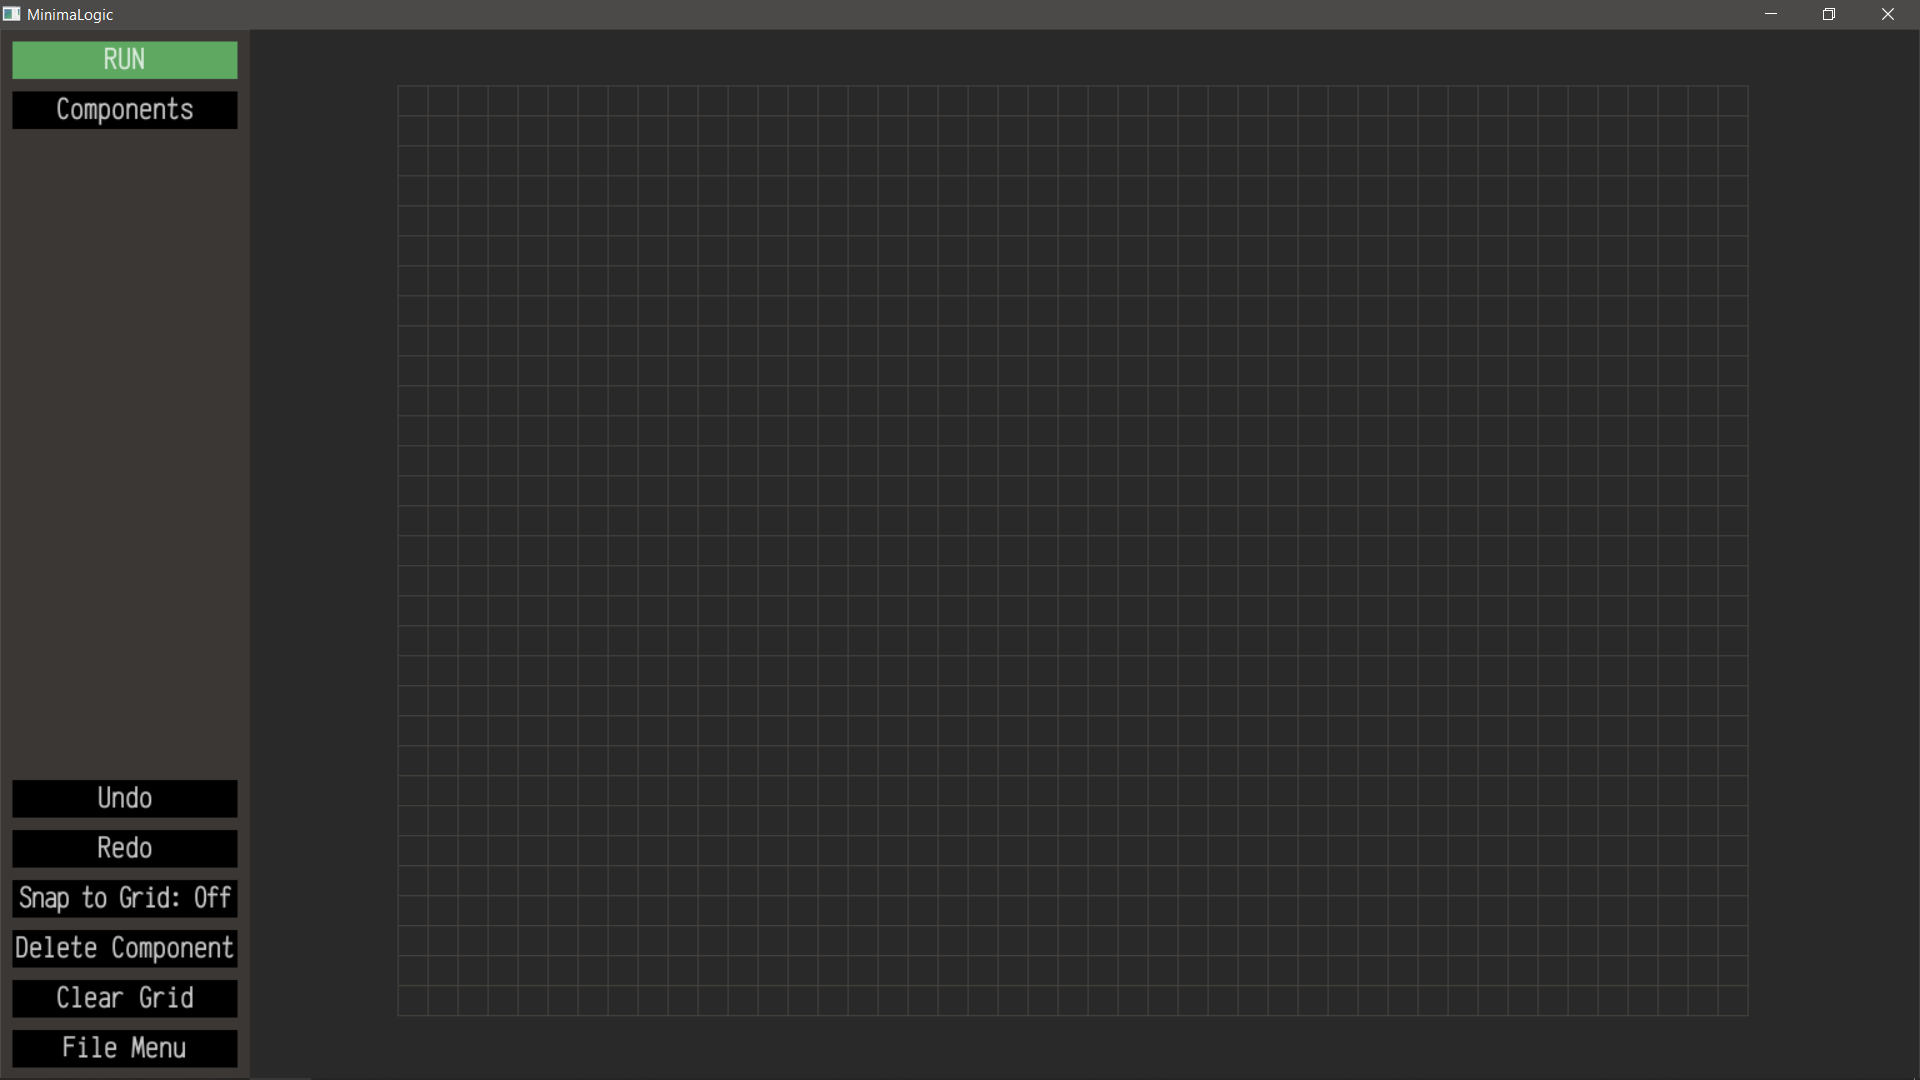
\includegraphics[width=0.8\textwidth]{graphics/initial_screen.png}
    \caption{Initial / Starting Screen}
\end{figure}
\begin{figure}[H]
    \centering
    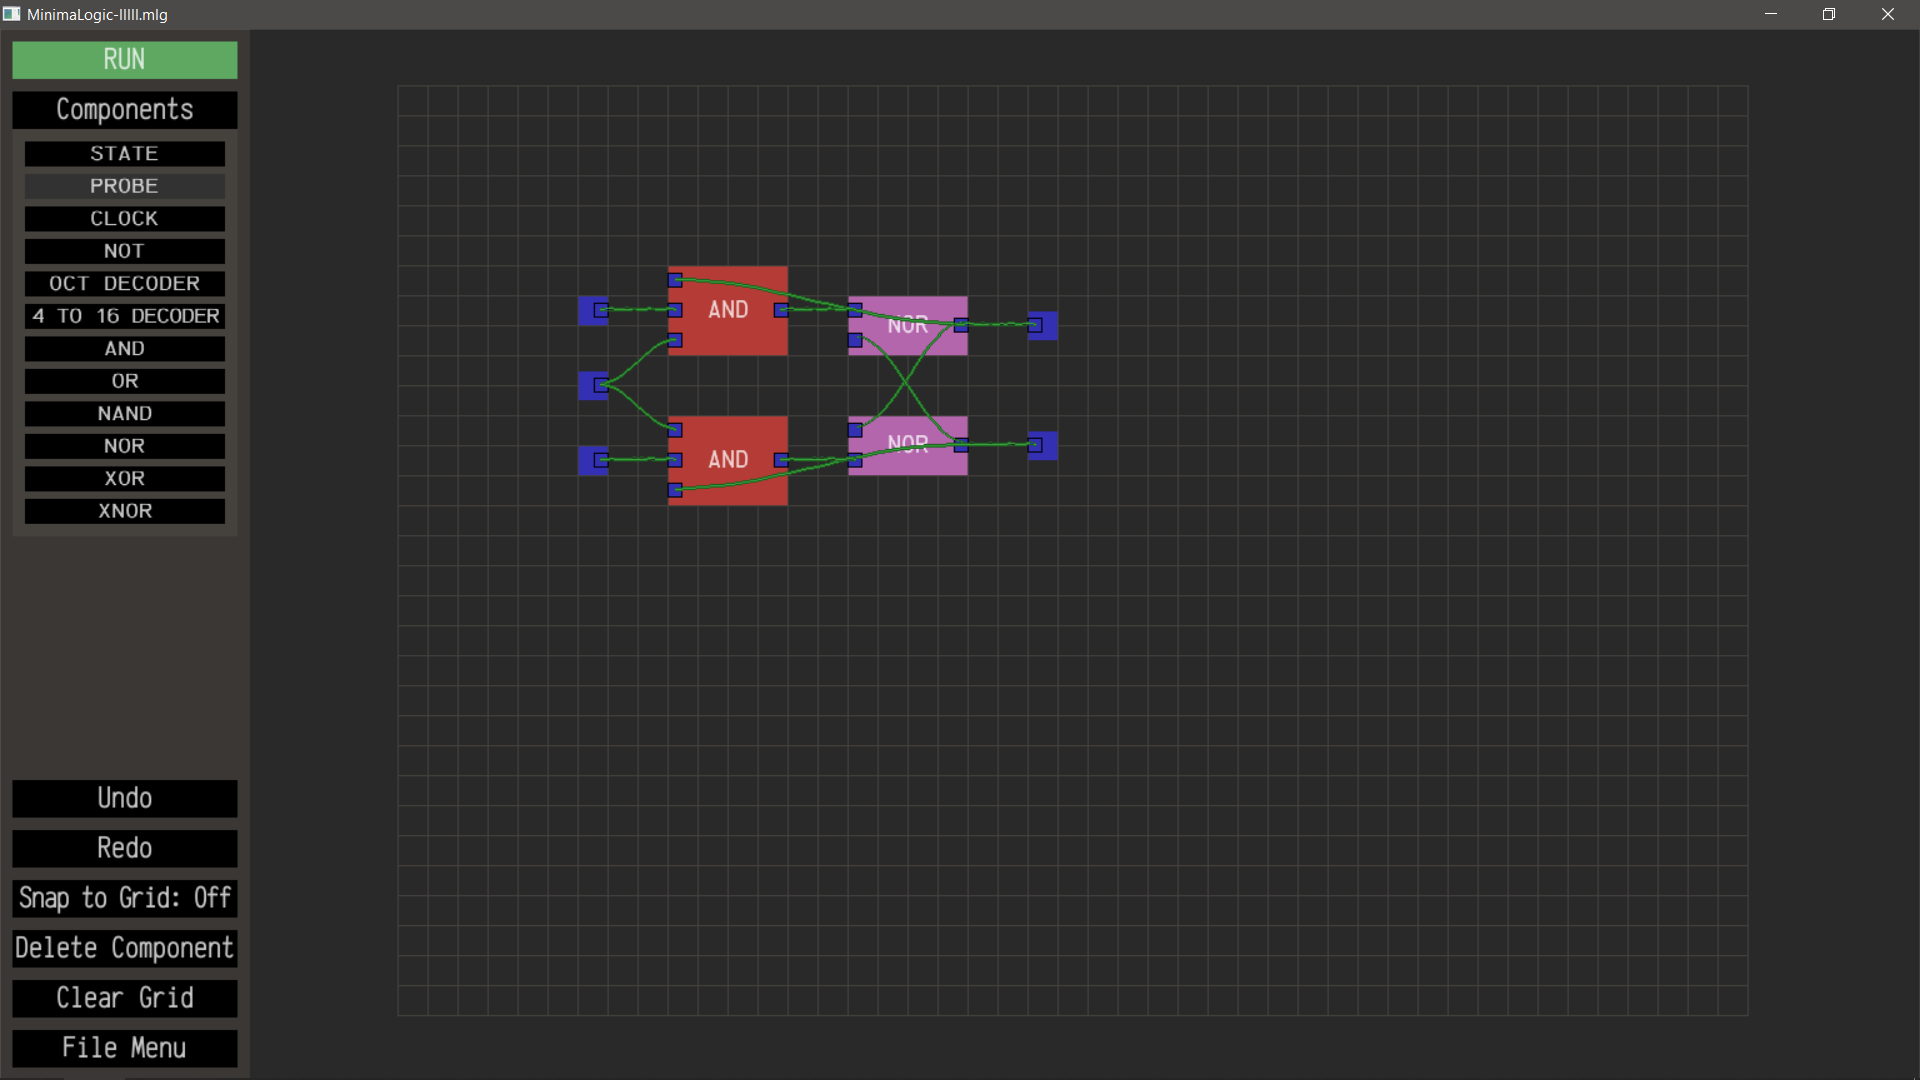
\includegraphics[width=0.8\textwidth]{graphics/jkff_normal.png}
    \caption{Circuit in normal state (not simulated)}
\end{figure}
\begin{figure}[H]
    \centering
    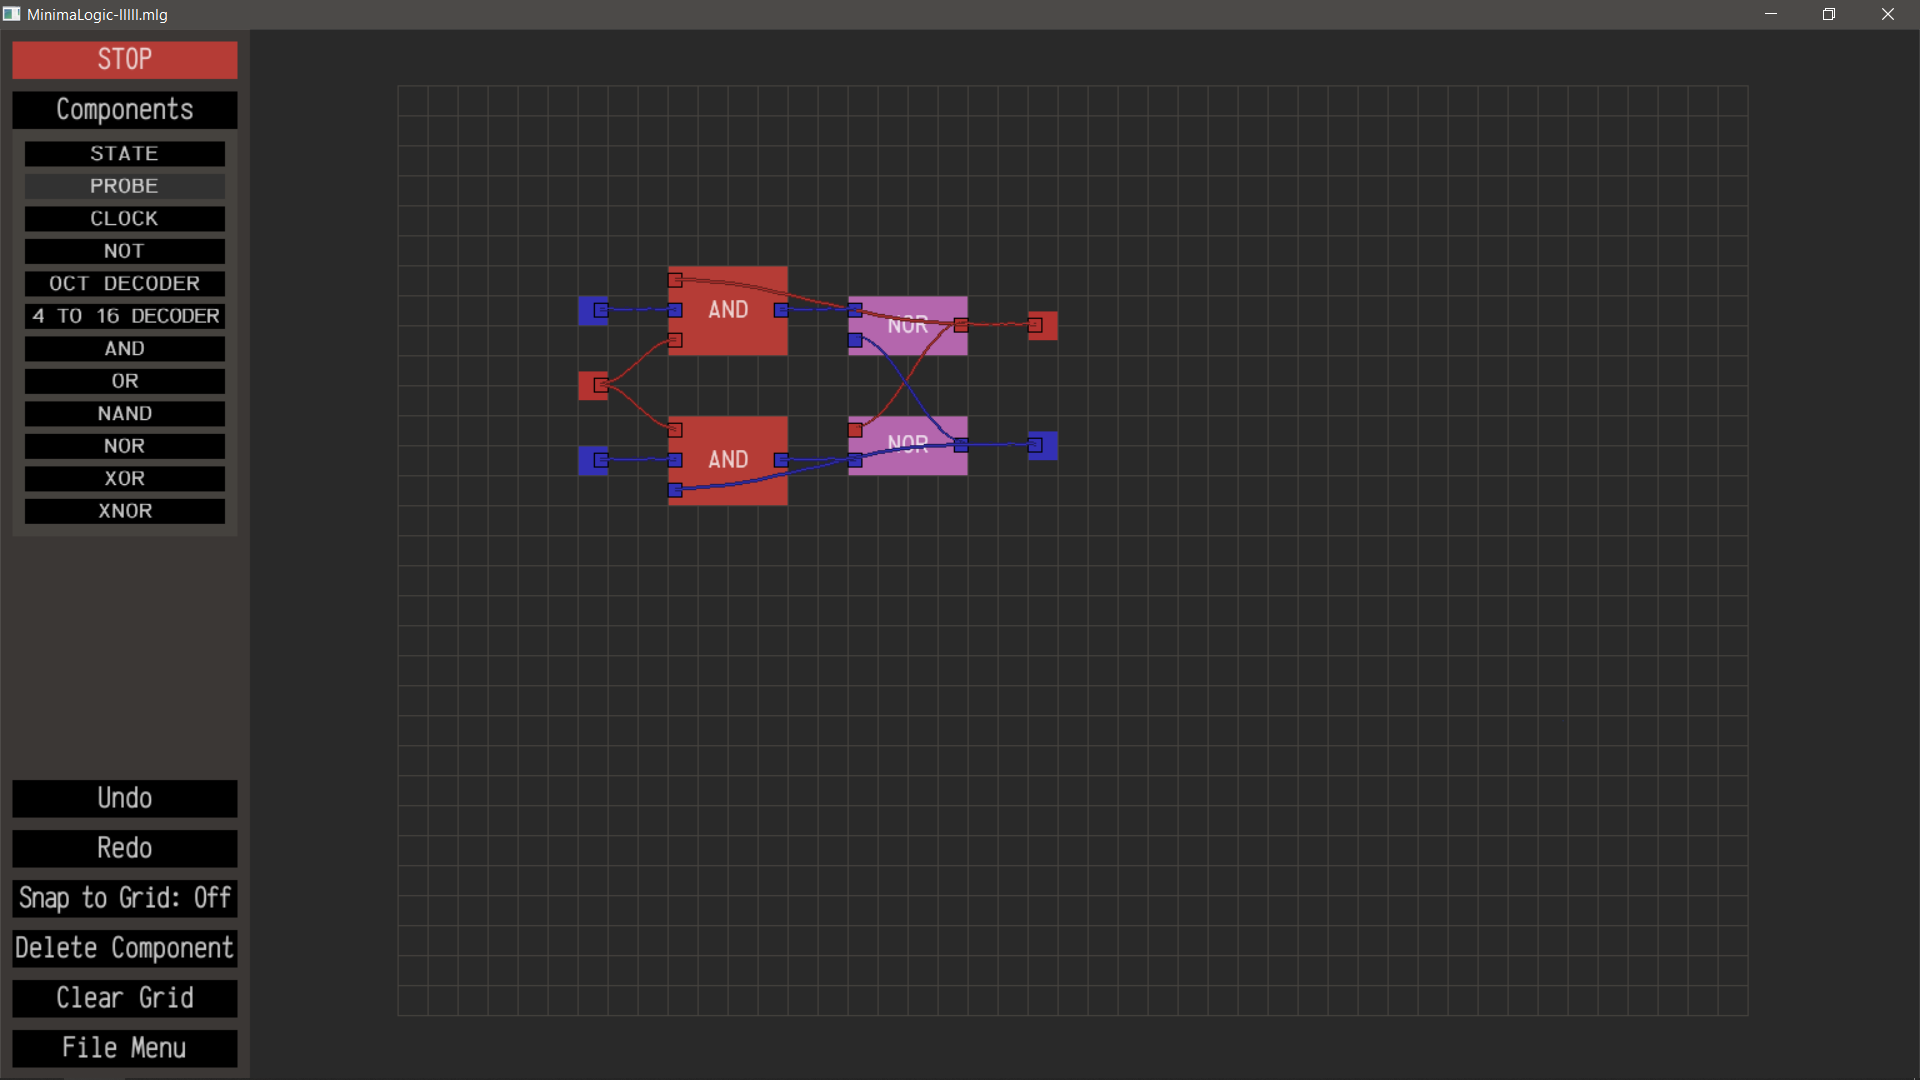
\includegraphics[width=0.8\textwidth]{graphics/jkff_simulating.png}
    \caption{Circuit being simulated}
\end{figure}
\begin{figure}[H]
    \centering
    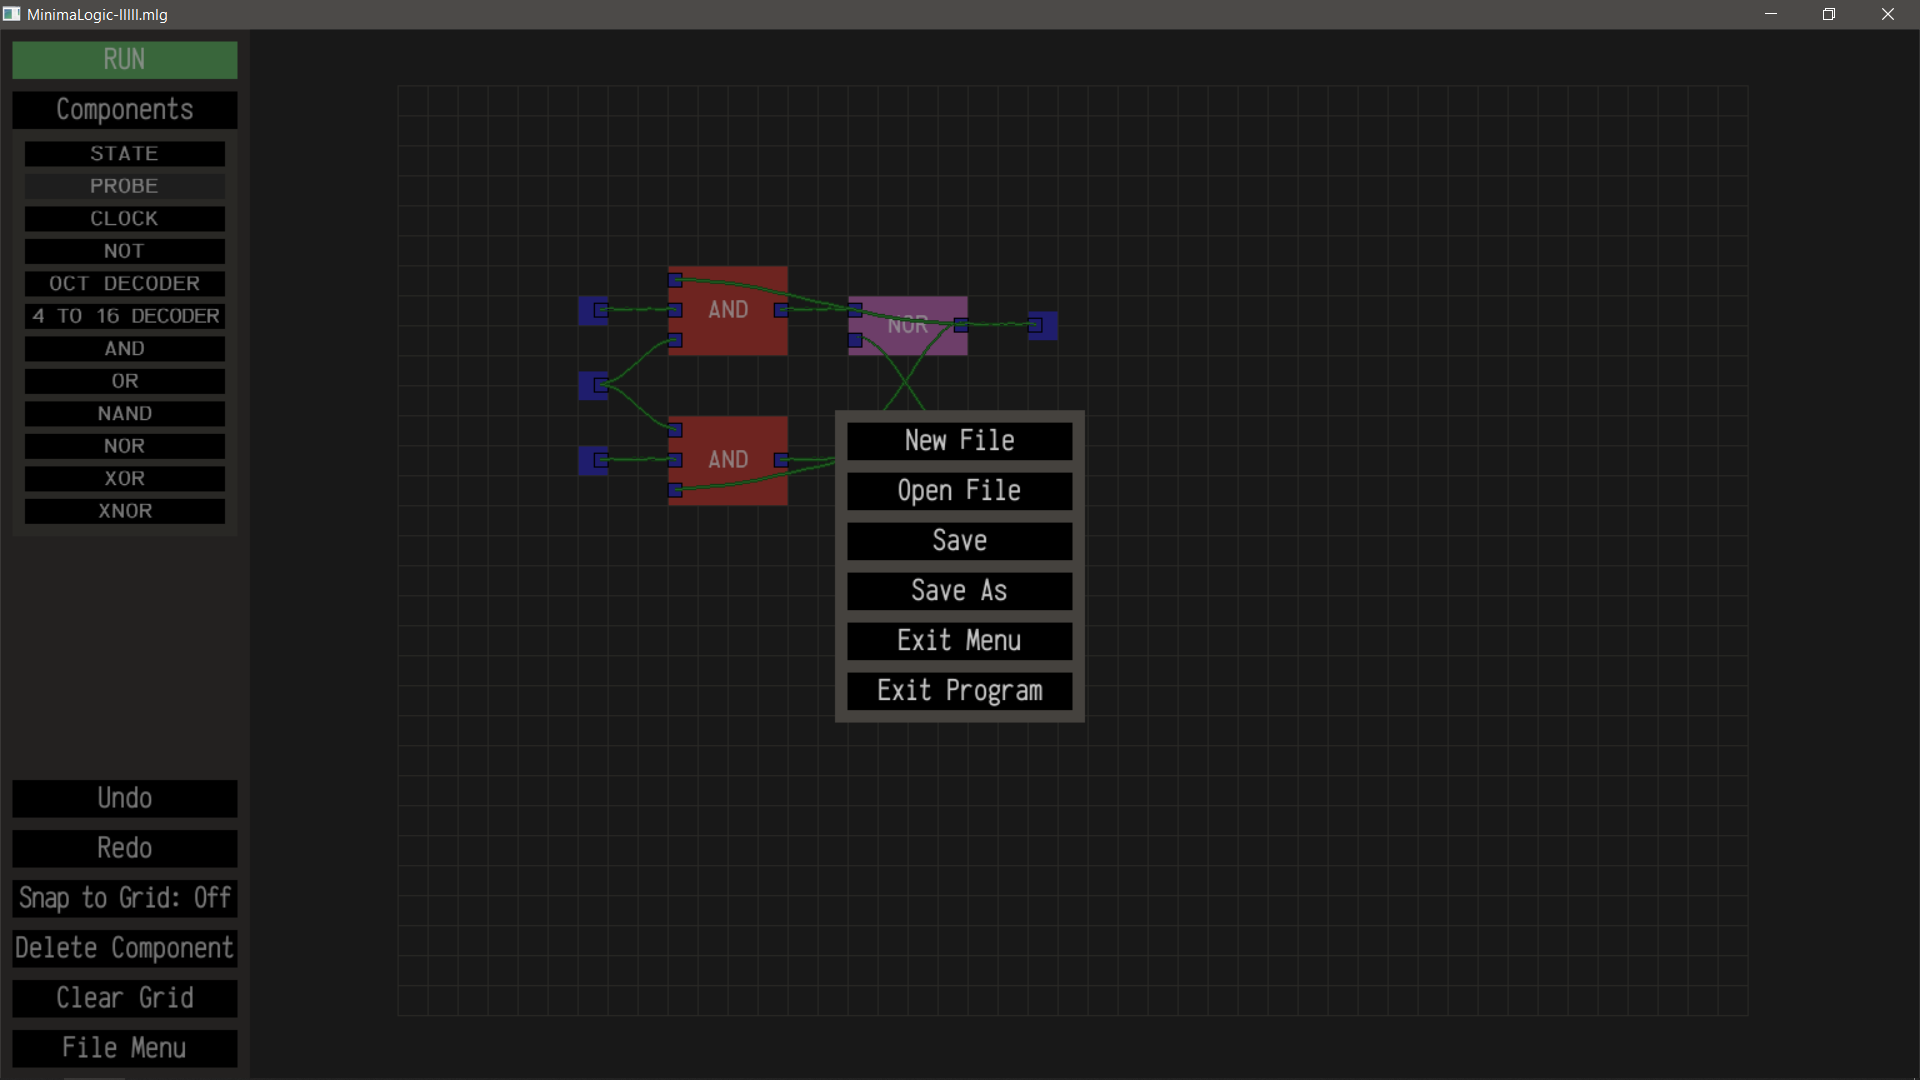
\includegraphics[width=0.8\textwidth]{graphics/file_menu.png}
    \caption{File Menu}
\end{figure}
\end{document}
